\chapter{Physical aspects}

Atomic nuclei have multiple energy states, many of which are not stable, forcing them to release some of their energy in order to reach a stable state. One decay however does not always lead to a direct transition into a stable state, it may even require the atom to change into another depending on what way it has released its energy. On the other hand, radiation is not only produced when atoms decay, it is constantly raining down upon us from the cosmos, this kind of radiation can also be detected with a CosmicWatch, making it also necessary to explore. This chapter aims to provide an overview of some of the mechanisms through which nuclei reach stable states and what cosmic radiation is. Chapter \ref{chap:detection_methods} provides an overview of how this can be used to take interesting measurements with CosmicWatch.

\section{Radioactivity}

It is first necessary to understand the concept of activity. Not all atoms take the same time to decay, each atom has its own constant $\Gamma$ which determines how likely it is to decay per unit of time. If one has an initial total of $N_0$ atoms, after a while it will be reduced due to the constant decay of atoms in the sample, this rate of change is given by the universal law of radioactive decay.
\begin{equation}
    \frac{dN(t)}{dt} = -\Gamma N(t)
\end{equation}

From this, it is easy to find that the number of remaining unstable atoms follows an exponential law
\begin{equation}
    N(t) = N_0 e^{-\Gamma t}
\end{equation}

The activity $A(t)$ of a radioactive source is given by how many decays occur per unit of time. This can be therefore obtained by multiplying the number of atoms $N(t)$ by the probability of decay per unit of time $\Gamma$.
\begin{equation}
    A(t) = \Gamma N_0 e^{-\Gamma t}
\end{equation}

The most common units for activity are the \textit{curie} (Ci) and the \textit{becquerel} (Bq), a becquerel represents one disintegration per second, while a curie represents $3.7\times10^{10}$ disintegrations per second ($\approx$ the activity of one gram of $^{226}Ra$). Under these definitions, the conversion between these units is given by the following relation:
\begin{eqnarray}
    1 \text{~Bq} = 2.703\times10^{-11} \text{~Ci}
\end{eqnarray}

The time constant $\Gamma$ is often expressed in terms of the atom's lifetime $\tau$ under the relation $\Gamma=1/\tau$. This means that $\tau$ is the time it takes to reduce a sample of $N_0$ by a factor of $1/e$, clearly $N(\tau)=N_0e^{-\Gamma \tau} = N_0/e$. On the other hand there also exists a constant called half-life $T_{1/2}$, which represents the time it takes to reduce the sample by half, Sodium 22 for example has a half-life of 2.605 years. They can both be related by doing $T_{1/2} = \ln (2)\tau$ \cite{knoll2010radiation}.

\subsection{Gamma emission}

\begin{figure}
  \centering
  \begin{subfigure}[t]{0.45\textwidth}
    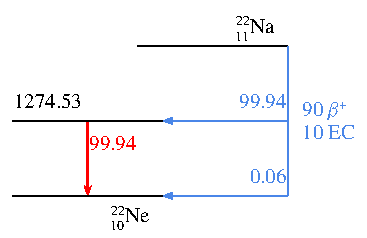
\includegraphics[width=\textwidth]{physical_aspects/22Na-decay.pdf}
    \caption{\label{sfig:22Na}}
  \end{subfigure}
  \begin{subfigure}[t]{0.425\textwidth}
    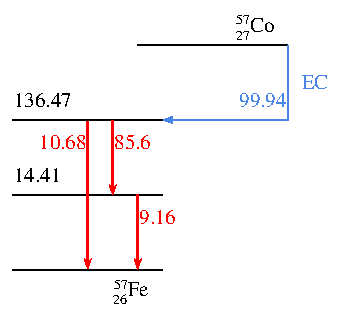
\includegraphics[width=\textwidth]{physical_aspects/57Co-decay.pdf}
    \caption{\label{sfig:57Co}}
  \end{subfigure}
  \medskip
  \centering
  \begin{subfigure}[t]{0.425\textwidth}
    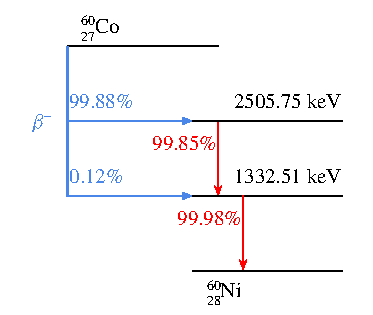
\includegraphics[width=\textwidth]{physical_aspects/60Co-decay.pdf}
    \caption{\label{sfig:60Co}}
  \end{subfigure}
  \begin{subfigure}[t]{0.425\textwidth}
    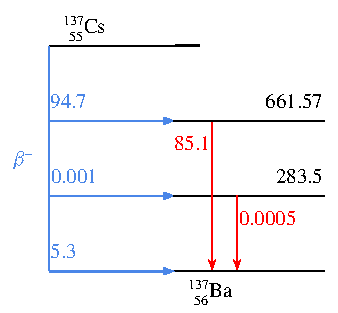
\includegraphics[width=\textwidth]{physical_aspects/137Cs-decay.pdf}
    \caption{\label{sfig:137Cs}}
  \end{subfigure}
  \caption{\label{fig:decay_schemes}Decay schemes for some isotopes used while testing the CosmicWatch. Only the main decay channels are included for clarity and simplicity. Energies [\unit{\kilo\eV}] for every level are shown in black. Branching ratios and decay mechanisms are shown in \textcolor{blue}{blue}. Gamma decays are represented with a \textcolor{red}{red} arrow also with its corresponding branching ratio.}
\end{figure}

Unstable nuclei have multiple channels to release their energy through, the conditions that determine what channels an atom can use are not studied here, but rather the subsequent effects of such channels. An atom can decay by emitting gamma rays, alpha particles, neutrons, or protons, it can also undergo beta $\beta^{\pm}$ decay, Internal Conversion, and Electron Capture among others. This work will focus on beta decay and Electron Capture since these are the preferred channels of decay of the radioactive sources used to test CosmicWatch.

\subsubsection{Beta decay}

There are two types of beta decay, they are represented by the following reaction schemes:
\begin{align}
  \beta^+ &:=~ ^A_ZX \rightarrow ~ ^A_{Z-1}Y + e^+ + \nu \\
  \beta^- &:=~ ^A_ZX \rightarrow ~ ^A_{Z+1}Y + e^- + \bar{\nu}
\end{align}

Where the symbols follow the nuclear notation, $X$ and $Y$ represent the initial and final elements, $A$ is the atomic number, $Z$ the nuclear charge, $e^{\pm}$ are a positron or electron, and $\nu/\bar{\nu}$ are a neutrino/antineutrino, Fig. \ref{fig:decay_schemes} shows some examples of these processes. Note for instance the case of $^{22}_{11}$Na Fig. \ref{sfig:22Na}, it undergoes $\beta^+$ $90\%$ of the time it decays, by the nuclear notation one can tell that the initial and final elements are Sodium and Neon respectively. In this process, a proton turns into a neutron, which is why the product element has $Z=11-1=10$ while maintaining $A=22$. It is important to also note that the total charge has to be conserved after the reaction occurs, which is why a positron $e^+$ is produced.

Alongside the positron/electron, a neutrino/antineutrino is ejected from the nucleus which, due to its extremely small interaction probability with matter, can not be detected. However, the negligible neutrino/antineutrino-matter interactions do not mean that their presence in the reaction does not have effects. The energy of the system also has to be conserved, since the particles $e^{\pm}$ and $\nu/\bar{\nu}$ are all ejected from the nucleus, higher or smaller portions of the total energy can be taken by the neutrino/antineutrino, which leaves multiple possible energy values for the positron/electron, resulting in continuous energy spectra.

\begin{figure}[H]
    \centering
    \begin{subfigure}[t]{0.45\textwidth}
      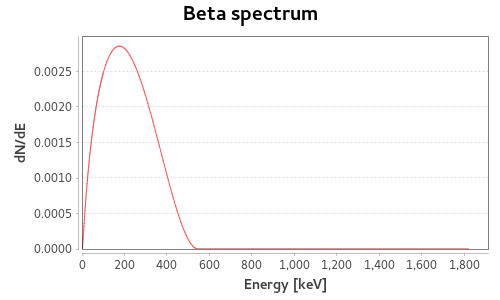
\includegraphics[width=\textwidth]{physical_aspects/22Na-beta-spectrum.jpg}
      \caption{\label{sfig:22Na_beta_spectra}}
    \end{subfigure}
    \begin{subfigure}[t]{0.45\textwidth}
      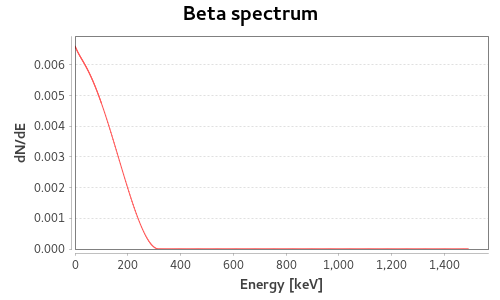
\includegraphics[width=\textwidth]{physical_aspects/60Co-beta-spectrum.jpg}
      \caption{\label{sfig:60Co_beta_spectra}}
    \end{subfigure}
    \caption{\label{fig:beta_spectra}positron/electron energy spectra for  \subref{sfig:22Na_beta_spectra} $^{22}$Na $(\beta^+)$ and  \subref{sfig:60Co_beta_spectra} $^{60}$Co $(\beta^-)$. Taken from \cite{IAEA}.}
\end{figure}

\subsubsection{Electron Capture}

The process of Electron Capture is analogous to $\beta^+$ decay, here an electron from de $K$ shell (or $L$, $M$, \dots) is captured by a proton in the nucleous, which then turns into a neutron while emitting a neutrino with a characteristic energy. The effect of this decay in the nucleous is the same as in $\beta^+$ (Z, A)$\rightarrow$(Z-1, A). The decay scheme is represented below:

\begin{equation}
  \text{EC} :=~ p + e^- \rightarrow ~ n + \nu
\end{equation}

Since this process leaves a vacancy in the lower shells of the electron cloud, an electron in an upper shell can decay to fill the space, resulting in the emission of characteristic X-rays.

\subsection{Light-matter interactions}

This section shows a review of the most important processes that govern gamma-ray interactions with matter, them being photoelectric effect, Compton scattering, and pair production.

\subsubsection{Compton scattering}

\subsubsection{Lineal attenuation coeficient}

\section{Cosmic Radiation}

\section{Particle interactions with matter}